\section{Introduction}

Introduce something great from \cite{Cook_Spitler_2021}

The segment response of \autoref{one_borehole_sr}...

\begin{figure}[hbt!]
  \centering
  \includegraphics[width=0.7\textwidth]{one_borehole_sr.pdf}
  \caption{The segment response of one borehole}
  \label{one_borehole_sr}
\end{figure} 

Now the \autoref{two_boreholes}...

\begin{figure}[hbt!]
     \centering
     \begin{subfigure}[b]{0.4\textwidth}
         \centering
         \includegraphics[width=\textwidth]{two_borehole_sr.pdf}
         \caption*{}
     \end{subfigure}
     \begin{subfigure}[b]{0.4\textwidth}
         \centering
         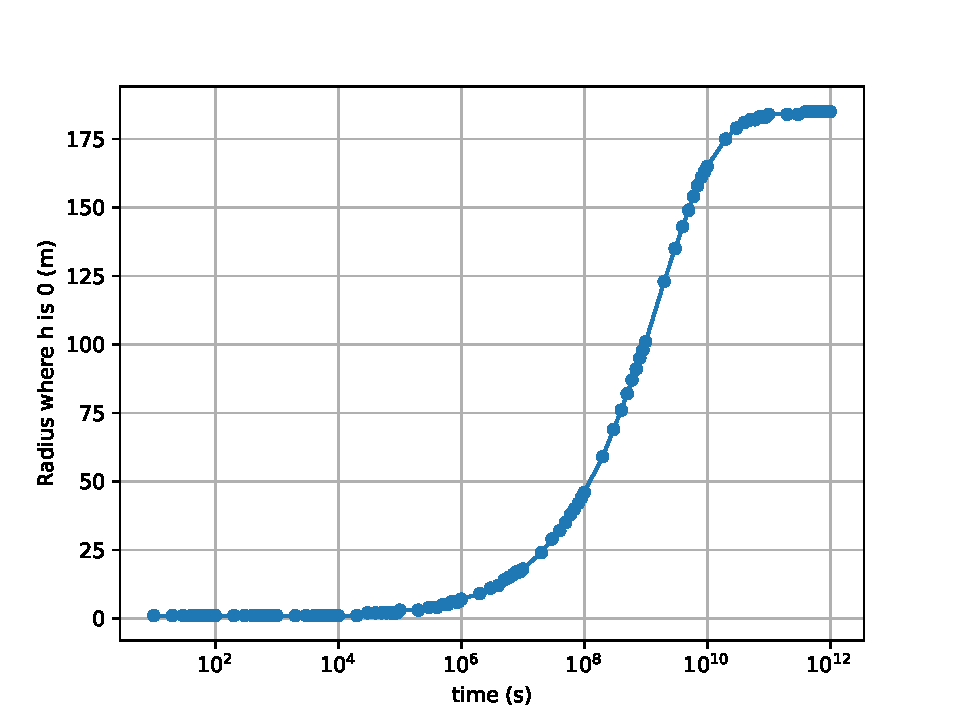
\includegraphics[width=\textwidth]{segment_nonresponse.pdf}
         \caption*{}
     \end{subfigure}
     \caption{The segment response of two boreholes and the distance of no response}
     \label{two_boreholes}
\end{figure} 

